%%%%------------------------------------------------
%
%  Include for chapter one of dissertation: introduction
%
%%%%------------------------------------------------
\section{Context}

Since the advent of the 'Digital Age' and the ability of computers to copy and
reproduce information for a negligible cost, the amount of information
available to researchers has been increasing drastically.  B-C Bj\"{o}rk (2009)
estimates that approximately 1.4 Million papers were published in the year 2006
alone\cite{bjork2009}. Moreover, the growing popularity of Open Access
publishing (making papers available to readers for free online\cite{Suber2012})
across most scientific disciplines\cite{bjork2009}\cite{harnad2004comparing} is
providing scientists and researchers with an even larger volume of information
to be processed. As available information increases, relevant material becomes
progressively more difficult to find manually and the need for an automated
information retrieval tool more apparent. The problem is even more vital for
General Practitioners. Goldacre (2008:97) points out that ``there have been an
estimated 15 million medical academic articles published so far, and 5000
journals published every month... picking out what's relevant is a gargantuan
task."\cite{goldacre2008bad}.

To assist in information processing and knowledge acquisition within the domain
of scientific research, a new web-based tool named Partridge was designed. Its
creation and implementation are discussed in this document.

\section{Background}

\subsection{ Related Works }

There are already a large number of information retrieval and recommendation
systems for scientific publications. A selection of these systems were
evaluated to find out which features work well and to identify their
shortcomings.

Several online search systems specifically index scientific papers and other
publications. One of the most publicised and well known paper search systems is
Google Scholar (\url{http://scholar.google.com}).  As can be seen in Figure
\ref{fig:scholar_basic}, This is an adaptation of Google's general search
engine to specifically index and search scientific papers.  Google offers
advanced query options specific to Scholar that allow searching by author, year
and for words that occur only in the document title as shown in figure
\ref{fig:scholar_advanced}. Whilst this does deal with the problem of
`information overload' by providing fine control over the information returned
from searches,  the user is still required to have a very good idea of what
they are looking for in terms of keywords and/or specific authors. It is
possible that a user would not know what they are looking for until they've
seen it. Even if the user has a set of keywords to search for, they can only
search the title of the paper or the content as a whole. This means that users
who want to find a particular phrase within a CoreSC part of the paper (e.g.
only look for this phrase in the `Result' section of the paper) are unable to
get results at their desired level of detail.

\begin{figure}[!hbt]
        \centering
        \begin{subfigure}[b]{0.50\textwidth}
                \centering
                
\includegraphics[width=\textwidth]{images/googlescholar_front.png}
                \caption{Google Scholar's General front page}
                \label{fig:scholar_basic}
        \end{subfigure}%
        \begin{subfigure}[b]{0.50\textwidth}
                \centering
                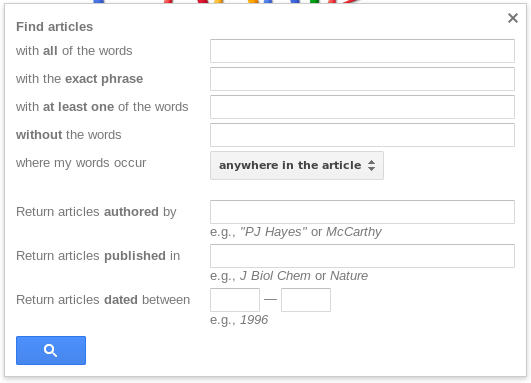
\includegraphics[width=\textwidth]{images/googlescholar_advanced.png}
                \caption{Advanced search features}
                \label{fig:scholar_advanced}
        \end{subfigure}

        \caption{Google Scholar's user interface}
        \label{fig:scholar_interface}
\end{figure}

Social citation and recommendation engines also provide a partial solution to
the `information overload' problem.  Services like Goodreads
(\url{http://www.goodreads.com/}) and CiteUlike
(\url{http://www.citeulike.org/}) allow you to register your interest in
specific authors and subjects. This allows the sites to build up a profile of
the sorts of materials that you might be interested in and provide lists of
recommendations as in Figure \ref{fig:social_indexes}.

\begin{figure}[!hbt]
        \centering
        \begin{subfigure}[b]{0.50\textwidth}
                \centering
                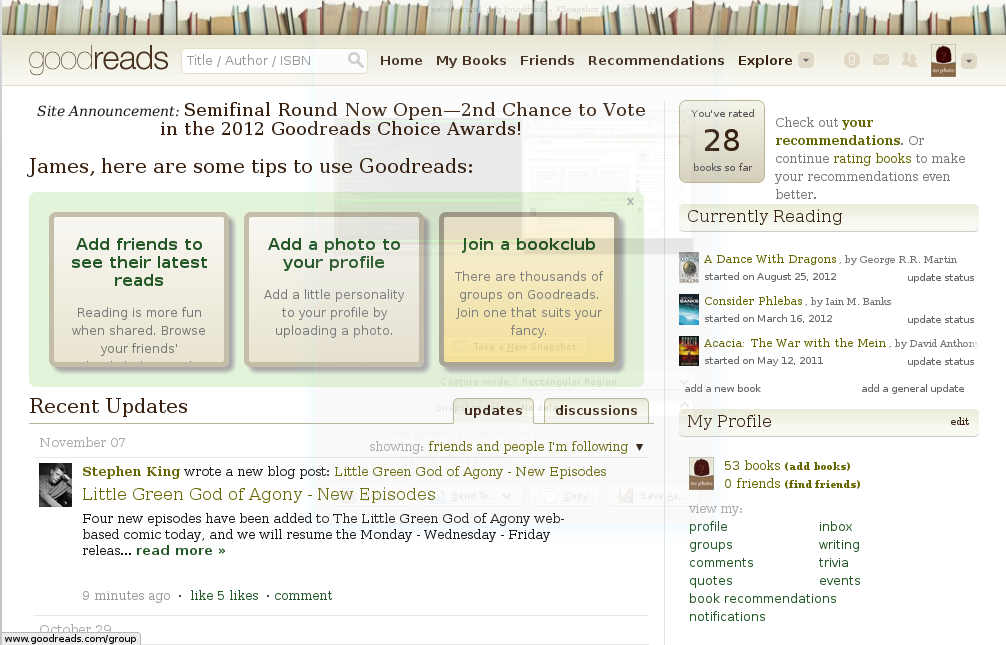
\includegraphics[width=\textwidth]{images/goodreads_index.png}
                \caption{Goodreads user profile page}
                \label{fig:goodreads_index}
        \end{subfigure}%
        \begin{subfigure}[b]{0.50\textwidth}
                \centering
                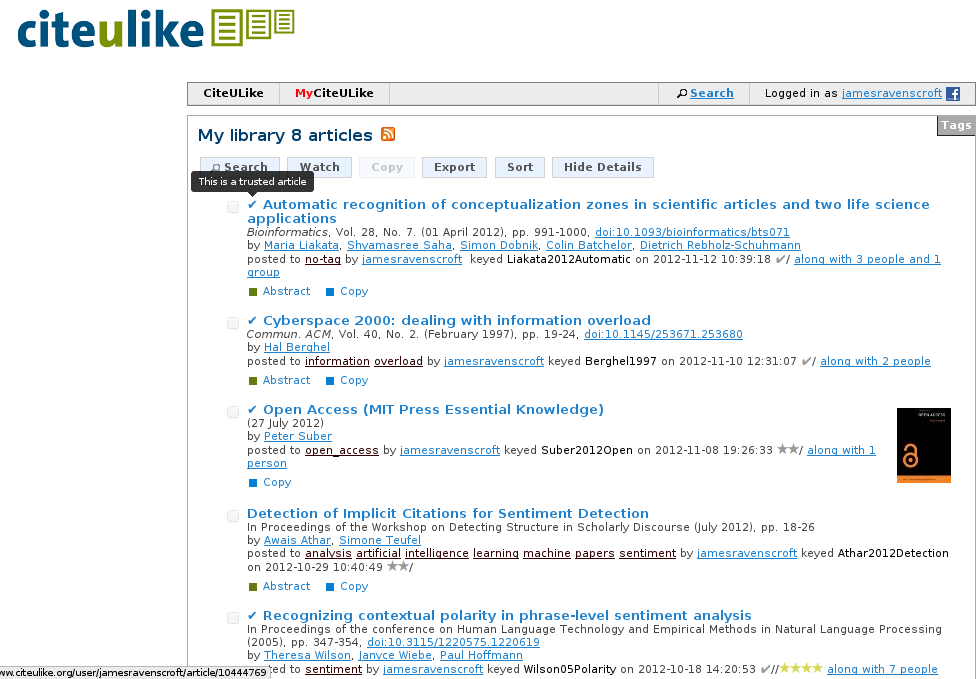
\includegraphics[width=\textwidth]{images/citeulike_index.png}
                \caption{a CiteULike user profile page}
                \label{fig:citeulike_index}
        \end{subfigure}

        \caption{Goodreads and citeulike social recommendation systems}
        \label{fig:social_indexes}
\end{figure}

These systems have the ability to make recommendations to the user without
requiring specific keywords or search terms. They do this by learning the
user's profile and taking into account the preferences of their 'friends' and
their browsing history. However, the above-named systems do not take into
account the content of the paper or book. They only deal with metadata as can
be seen in Figure \ref{fig:social_searches}. This means that important
discriminatory information that could be contained within the actual document
content is overlooked completely. 

\begin{figure}[!hbt]
        \centering
        \begin{subfigure}[b]{0.50\textwidth}
                \centering
                
\includegraphics[width=\textwidth]{images/goodreads_search.png}
                \caption{Goodreads advanced search page}
                \label{fig:goodreads_search}
        \end{subfigure}%
        \begin{subfigure}[b]{0.50\textwidth}
                \centering
                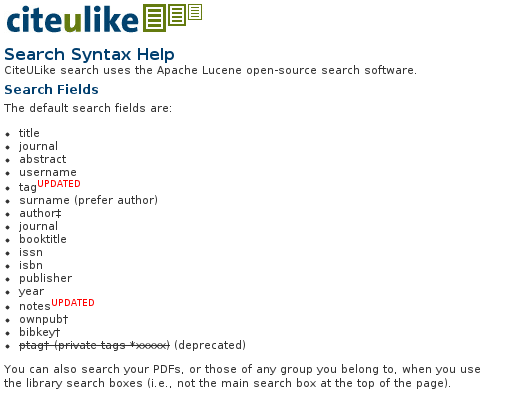
\includegraphics[width=\textwidth]{images/citeulike_search.png}
                \caption{CiteULike advanced search options}
                \label{fig:citeulike_search}
        \end{subfigure}

        \caption{Goodreads and citeulike search only deal with metadata.}
        \label{fig:social_searches}
\end{figure}

None of these systems make full use of the content within the research papers
that they index. Those systems with filtering and recommendation capabilities
rely upon users and their activities to provide discriminatory information
between papers and facilitate `intelligent' behaviour. It is hoped that by
making full use of the content within scientific papers, Patridge will offer a
novel, reliable way of displaying relevant papers to users.

\section{ Literature Review}

\subsection{Natural Language Processing}

Natural Language Processing (NLP)  is a branch of Artificial Intelligence that
enables the automated extraction of meaningful information from texts written
in human languages such as French or English. Liddy (2001) defines Natural
Language Processing as:

\begin{quotation} 
A theoretically motivated range of computational techniques for analyzing and
representing naturally occurring texts at one or more levels of linguistic
analysis for the purpose of achieving human-like language processing for a
range of tasks or applications \cite{liddy2001natural}.  
\end{quotation}

Over the last 60 years, NLP has been used in a wide variety of applications
such as automated translation between languages\cite{hutchins2004first}, the
engineering of systems for querying databases using natural languages
\cite{rao2010natural} and for building `chatterbot' systems designed to
communicate with their users in a human-like way\cite{Alfonsi2006}.
More recently, NLP has been used for text classification purposes such as
classifying emotions within phrases and sentences \cite{Wilson05Polarity} and
even within suicide notes \cite{citeulike:11077287}.


\subsection{CISP, CoreSC and SAPIENTA}

Liakata \emph{et al.} (2012) describe a system for automatically processing and
classifying sentences in a research paper according to the scientific concept
they describe (e.g. a sentence can be categorised as a hypothesis, background
information, a method or similar)\cite{citeulike:10444769}. SAPIENTA
(\url{http://www.sapientaproject.com}) is a machine learning application,
trained using a corpus of physical chemistry and biochemistry research papers
that were pre-processed and annotated using Core Information about Scientific
Papers (CISP)\cite{LIAKATA10.644}. 

CISP, Soldatova and Liakata (2007), is a way to formally represent core
scientific concepts (CoreSC), e.g. background, hypothesis, method etc., that
should be present in the articles in a logical
ontology\cite{soldatova2007ontology}. Subsequent work implements this set of
concepts as a three layered sentence based annotation scheme (CoreSC scheme)
where annotations are encoded in Extended Markup Language
(XML)\cite{LIAKATA10.644}.

\section{Objectives}
\label{sec:objectives}
Partridge's main objective is to provide reading recommendations and
information retrieval for scientists and researchers. This should reduce the
amount of extraneous information that users have to read for themselves by
helping them find information specific to their interests more quickly.
Partridge will achieve this through the use of several existing techniques in
Natural Language Processing and utilisation of SAPIENTA as discussed above.

Partridge is designed to help and facilitate researchers and authors of
scientific papers in the following principal ways:

\begin{itemize}
\item The system should provide search within specific CoreSC regions of a given
paper. This would allow users to find the most relevant papers to them. For
example a user may search for "mass spectrometer" within the methodology
section of a paper.
\item Partridge should allow authors and rightsholders of scientific papers to
upload their papers to the system for inclusion into the search system. This
would give Partridge itself more utility and would make involved authors more
accessible.
\item The system should provide filtering of papers based upon their
specific domain (i.e. is the paper primarily concerned with methodology within
an experiment in chemistry or is it about ethics in psychological studies?) and
their result, whether the paper yielded positive, negative or inconclusive
evidence for a hypothesis. 
\item Depending upon the time constraints of the
project, it was hoped that Partridge will also offer a user 'profiling' system
that provides recommendations for researchers based on their reading history.
This feature should help users find relevant papers more quickly or find
research that they may have otherwise overlooked.a
\end{itemize}

